\chapter{PV Panel Curves and simulation program} \label{ap:pvPanelCurves}

	This appendix shows the simulation curves of the photovoltaic panel static equation \eqref{eq:PVPanelModelModified}. It also shows listing \ref{lst:pvPanelCurves}, the Python program used to obtain those curves. The parameter values of the photovoltaic panels are denoted in table \ref{tab:panelParameters}.

\begin{figure}[h]
	\centering
	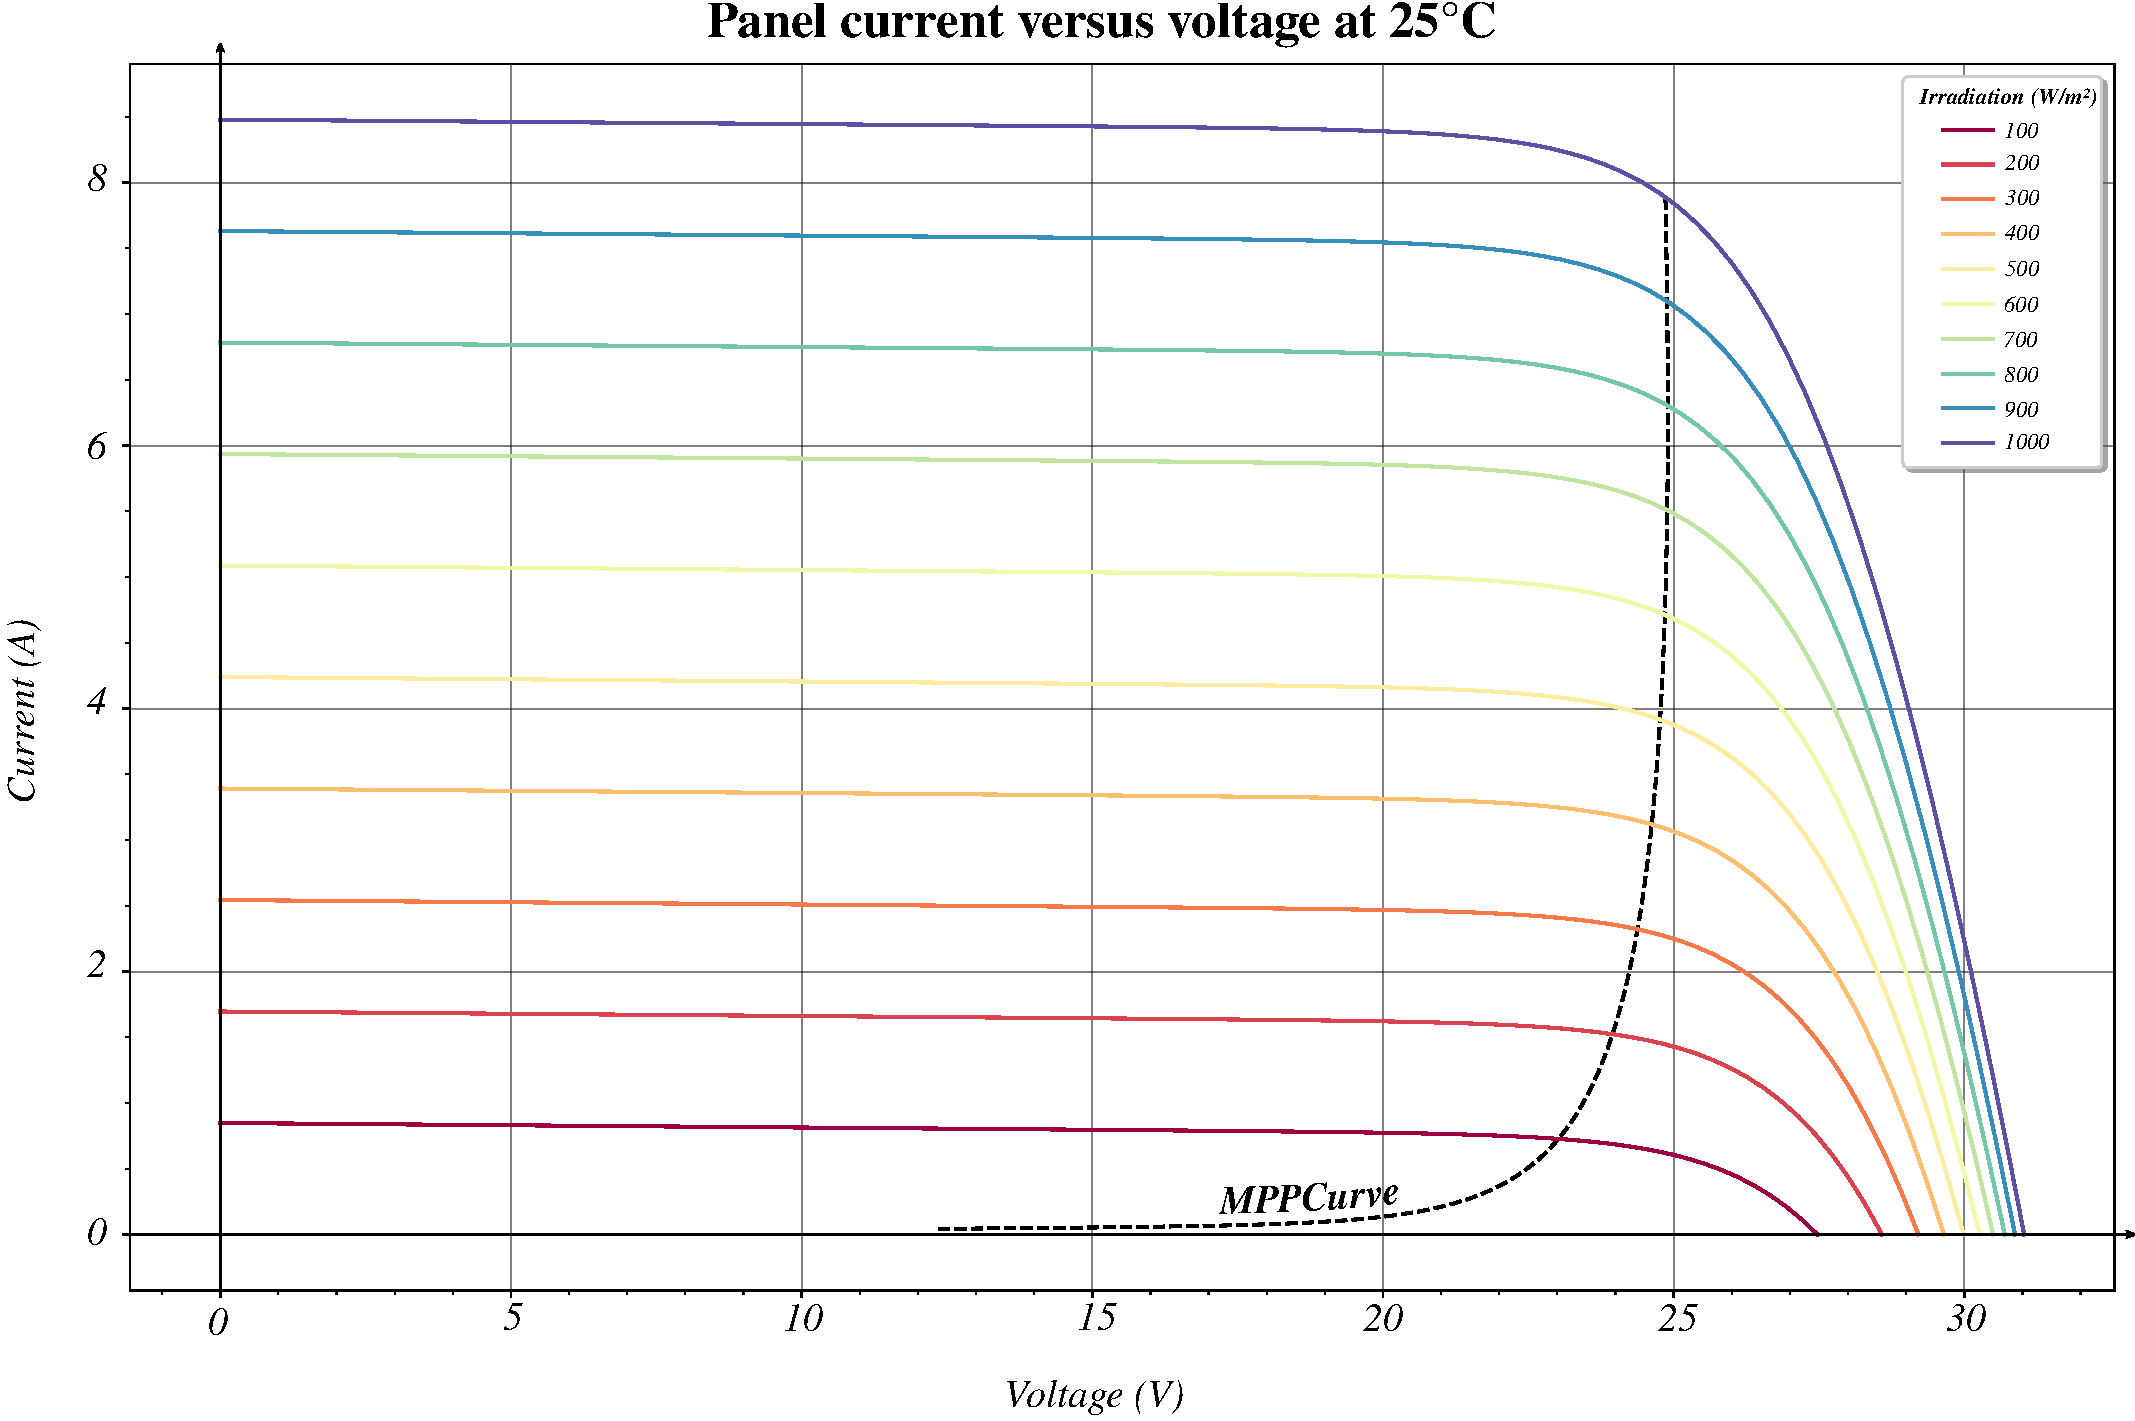
\includegraphics[angle = -90, width = 0.9\textwidth]{../images/pvPanelCurves/ivCurve.pdf}
	\caption{Panel transconductance (continuous) and MPP (dashed) curves with fixed temperature $\theta_{SRC}$ and varying irradiance.}
	\label{fig:ivCurve}
\end{figure}

	\lstinputlisting[caption = {Python PV panel simulation program developed to generate figures \ref{fig:ivCurve} to \ref{fig:pvCurveVaryingTemperature}}, label = {lst:pvPanelCurves}, style = prettyListing, language = Python]{../images/pvPanelCurves/mppTracking.py}
